\documentclass[../kl10.tex]{subfiles}
\graphicspath{{\subfix{../images/}}}

\renewcommand\tabularxcolumn[1]{m{#1}}% for vertical centering text in X column

\begin{document}

\section{Knock-Out durch Agatha Christie}
\noindent
\begin{minipage}[H]{0.8\textwidth}
  \textsc{Agatha Christie} (1890 – 1976) brachte ihre Romanfiguren am liebsten mittels Gift um die Ecke. Neben verschiedensten Alkaloiden wie Strychnin oder Morphium fand die weltbekannte Krimiautorin auch für Chloralhydrat als Mordmittel Verwendung. 
\end{minipage}
\hfill
\begin{minipage}[H]{0.19\textwidth}
  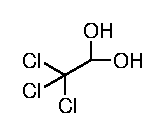
\includegraphics[width=0.7\textwidth]{2024/Abbildungen/Hydrat/Chloralhydrat.eps}
\end{minipage}


\enumaufgabe{\operator{Gib} den systematischen Namen nach IUPAC für Chloralhydrat \operator{an}.}
\solution{2,2,2-Trichlor-1,1-ethandiol oder 2,2,2-Trichlorethan-1,1-diol \ \ 1 P.}{1cm}

Chloralhydrat wurde dabei erstmals 1831 durch \textsc{Justus von Liebig} hergestellt. Die Synthese gelang durch die Oxidation von Ethanol mit Chlor zu Trichlorethanal und anschließende Hydratisierung. 

\enumaufgabe{\operator{Formuliere} die zur Herstellung von Chloralhydrat relevanten Reaktionsgleichungen.}
\solution{
\ce{C2H5OH + 4Cl2 -> CCl3CHO + 5HCl}\\
\ce{CCl3CHO + H2O -> CCl3CH(OH)2}\\
1,5 P. auf jede Reaktionsgleichung (1 P. auf Stoffchemie, 0,5 P. auf Stöchiometrie)\,
insg. 3 P.}{1.5cm}

Chloralhydrat gehört zur Stoffklasse der Hydrate, wie der Trivialname bereits verrät. Systematisch lässt sich die Verbindung allerdings auch als \textbf{X} Diol bezeichnen. Bei \textbf{X} handelt es sich um ein Adjektiv, das die relative Anordnung der Hydroxygruppen beschreibt. 
\enumaufgabe{\operator{Kreuze an}, was der passende Beriff für \textbf{X} ist. \solutiontext{1 P.}{}}
\renewcommand{\arraystretch}{2}
\begin{tabularx}{\textwidth}{|X|p{2.5cm}|X|p{2.5cm}|X|p{2.5cm}|}
    \hline
    vicinal & & geminal & \solutiontext{X}{} & isoliert & \\\hline
\end{tabularx}
\ \\ \ \\
Chloralhydrat dürfte nach der \textsc{Erlenmeyer}-Regel eigentlich gar nicht existieren. Diese besagt, dass Verbindungen, die an einem Kohlenstoff-Atom mehr als eine Hydroxygruppe tragen, instabil sind und zur Abspaltung von Wasser neigen. 

\begin{figure}[H]
    \centering
    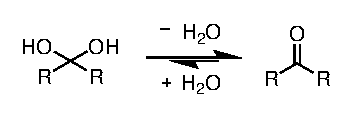
\includegraphics[width=0.37\textwidth]{2024/Abbildungen/Hydrat/2.eps}
\end{figure}

\enumaufgabe{\operator{Gib} einen möglichen Reaktionsmechanismus für die Umwandlung des Hydrats in die entsprechende Carbonylverbindung im sauren Milieu \operator{an}. Gehe von der oben angegeben allgemeinen Form des Hydrats mit den Resten R aus.}

\solution{
\begin{figure}[H]
    \centering
    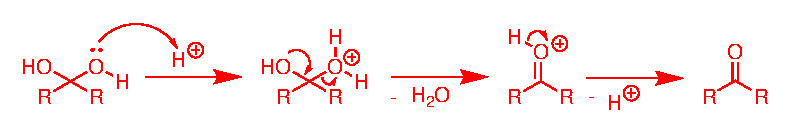
\includegraphics[width=0.8\textwidth]{2024/Abbildungen/Hydrat/Hydratbildung.eps}
\end{figure}
1 P. auf jedes Intermediat, jeweils 1 P. auf Protonierungs- und Deprotonierungsschritt, 1 P.  auf Kondensationsschritt\\
insg. 5 P.}{5cm}

Gemäß \textsc{Erlenmeyer} ist die Ursache für die Instabilität vieler Hydrate die deutlich höhere Bindungsenergie der C=O-Doppelbindung gegenüber der C-O-Einfachbindung und die gegenseitige Abstoßung der räumlich nah beieinander liegenden Sauerstoffsubstituenten. 

\enumaufgabe{\operator{Erläutere}, weshalb Chloralhydrat in wässriger Lösung entgegen der \textsc{Erlenmeyer}-Regel fast vollständig vorliegt.}

\solution{
Die drei Chlorsubstituenten (0,5 P.) in $\alpha$-Stellung erhöhen die Elektrophilie des Carbonylkohlenstoffs (0,5 P.) durch deren -I-Effekt (0,5 P.) derart, dass der nukleophile Angriff durch Wasser stark begünstigt wird (0,5 P.) und so das GGW verschiebt.\\
Anmerkung: Alternative sinnvolle Begründung unter thermodynamischen Gesichtspunkten soll ebenfalls korrekt bewertet werden.
\\
insg. 2 P.}{3cm}

Neben Chloralhydrat gibt es noch weitere Verbindungen, die sich der \textsc{Erlenmeyer}-Regel widersetzen. Weitere Beispiele sind in der folgenden Tabelle aufgeführt. 

\enumaufgabe{\operator{Gib} für jede Verbindung Effekte und Strukturmerkmale \operator{an}, die dafür verantwortlich sind, dass in wässriger Lösung hauptsächlich die Hydratform vorliegt. \operator{Ergänze} die Bezeichnung des Stoffes (Trivialname oder IUPAC-Name), sofern dieser fehlt.}

\renewcommand{\arraystretch}{1.7}
\solutiontext{}{\setlength{\extrarowheight}{5pt}}
\begin{tabularx}{\textwidth}{|L{3.5cm}|C{3.5cm}|X|}
    \hline
    \multirow{4}{*}{\solutiontext{Cyclopronanon (1 P.)}{}} & \multirow{4}{*}{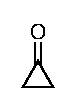
\includegraphics[width=0.05\textwidth]{2024/Abbildungen/Hydrat/Cyclopropanon.eps}} & \solutiontext{Bindungswinkel durch Dreiring beträgt $60^\circ$ (0,5 P.)}{}\\
    & & \solutiontext{sp$^2$-Hybridisierung erfordert eigentlich $120^\circ$ (0,5 P.)}{}\\
    & & \solutiontext{durch Hydratisierung ist Kohlenstoff sp$^3$-hybridisiert mit einem erforderlichen Winkel von $109,5^\circ$ (0,5 P.)}{}\\
    & & \solutiontext{geringere Abweichung vom idealen Bindungswinkel führt zu geringerer Ringspannung (0,5 P.)}{  }
    \\\hline
    \multirow{3}{*}{Ninhydrin} & \multirow{3}{*}{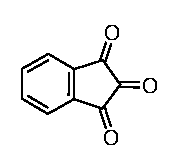
\includegraphics[width=0.17\textwidth]{2024/Abbildungen/Hydrat/Ninhydrin.eps}} & \solutiontext{elektronenziehende Carbonylgruppen, die -I-Effekt ausüben, in $\alpha$-Stellung (0,5 P.)}{}\\
    & & \solutiontext{Erhöhung der Elektrophilie des Carbonylkohlenstoffs (0,5 P.)}{}\\
    & & \solutiontext{Nukleophiler Angriff durch Wasser ist begünstigt (0,5 P.)}{\vspace{4cm}}
    \\\hline
    \solutiontext{Formaldehyd oder Methanal (1 P.)}{} & \multirow{3}{*}{
\includegraphics[width=0.09\textwidth]{2024/Abbildungen/Hydrat/Formaldehyd.eps}} & \solutiontext{H-Substituenten haben einen sehr geringen sterischen Anspruch, dadurch geringere sterische Hinderung der Sauerstoffatome (0,5 P.)}{}\\
    & & \solutiontext{kein $+$I-Effekt durch H-Substituenten, d.h. Carbonylkohlenstoff recht elektrophil (0,5 P.)}{}\\
    & & \solutiontext{Nukleophiler Angriff durch Wasser ist begünstigt (0,5 P.)}{\vspace{4cm}}
    \\\hline
    \solutiontext{Oxoessigsäure oder Glyoxalsäure (1 P.)}{} & \multirow{2}{*}{\includegraphics[width=0.15\textwidth]{2024/Abbildungen/Hydrat/Oxoessigsäure.eps}} & \solutiontext{elektronenziehende Carboxygruppe, die $-$I-Effekt ausübt, in $\alpha$-Stellung (0,5 P.)}{}\\
    & & \solutiontext{Erhöhung der Elektrophilie des Carbonylkohlenstoffs, Nukleophiler Angriff durch Wasser ist begünstigt (0,5 P.)}{\vspace{4cm}}
    \\\hline
\end{tabularx}\\\\
\solutiontext{Insg. 9,5 P.}{}

\newpage

\enumaufgabe{\operator{Markiere} bei Ninhydrin die Carbonylgruppe, die von Wasser nukleophil angegriffen wird.}
\solution{ \solutiontext{ 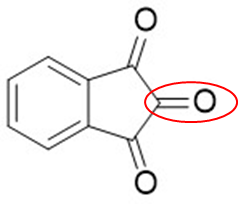
\includegraphics[width=0.2\textwidth]{2024/Abbildungen/Hydrat/L_g.png}}{ 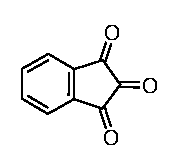
\includegraphics[width=0.2\textwidth]{2024/Abbildungen/Hydrat/Ninhydrin.eps}}
   1 P.
}{3cm}
\enumaufgabe{\operator{Zeichne} die Hydratform von Ninhydrin.}
\solution{
    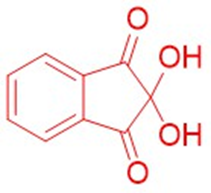
\includegraphics[width=0.2\textwidth]{2024/Abbildungen/Hydrat/L_h.png}1 P.
}{3cm}

\textsc{Agatha Christie}, die eine Ausbildung als Apothekerin absolvierte, wusste, dass Chloralhydrat in der richtigen (Über-)dosis tödlich wirkt. Tatsächlich wurde es lange Zeit als Schlafmittel und auch als Narkotikum eingesetzt. Ende des 19. Jahrhunderts begründete \textsc{Oskar Liebreich} die Wirkung von Chloralhydrat als Schlafmittel fälschlicherweise damit, dass es im Körper zu Chloroform (Trichlormethan) umgewandelt würde. Tatsächlich wird Chloralhydrat im Alkalischen in Chloroform und Formiat (Anion der Methansäure) gespalten. Eine Erklärung für die Wirkung auf den menschlichen Körper liefert diese Reaktion allerdings nicht. 

\enumaufgabe{\operator{Gib} einen möglichen Reaktionsmechanismus für die Spaltung von Chloralhydrat in Chloroform und Formiat \operator{an}.} 

\solution{\begin{figure}[H]
    \centering
    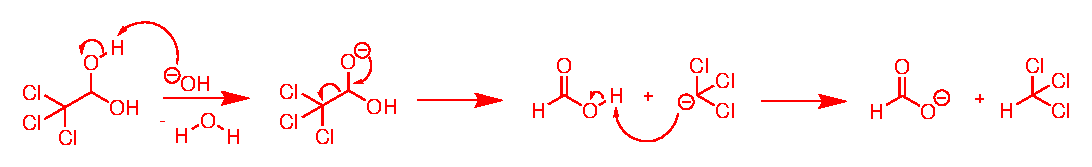
\includegraphics[width=\textwidth]{2024/Abbildungen/Hydrat/Chloralhydrat 1.eps}
\end{figure}
1 P. auf jede Spezies, jeweils 1. Punkt auf Deprotonierungsschritt, 1,5 P. auf Schritt mit C-C-Bindungsspaltung\\
9,5 P.}{6cm}

\newpage

Chloralhydrat dient auch als Ausgangsstoff für sogenannte Chloralosen. Diese finden nicht nur als Rattengift Verwendung. So zeigen die Aminderivate von $\alpha$-Chloralose eine antimikrobielle Wirkung. Um diesen Effekt zu untersuchen, führte eine Gruppe von Forschenden folgende Synthesesequenz durch: 

\begin{figure}[H]
    \centering
    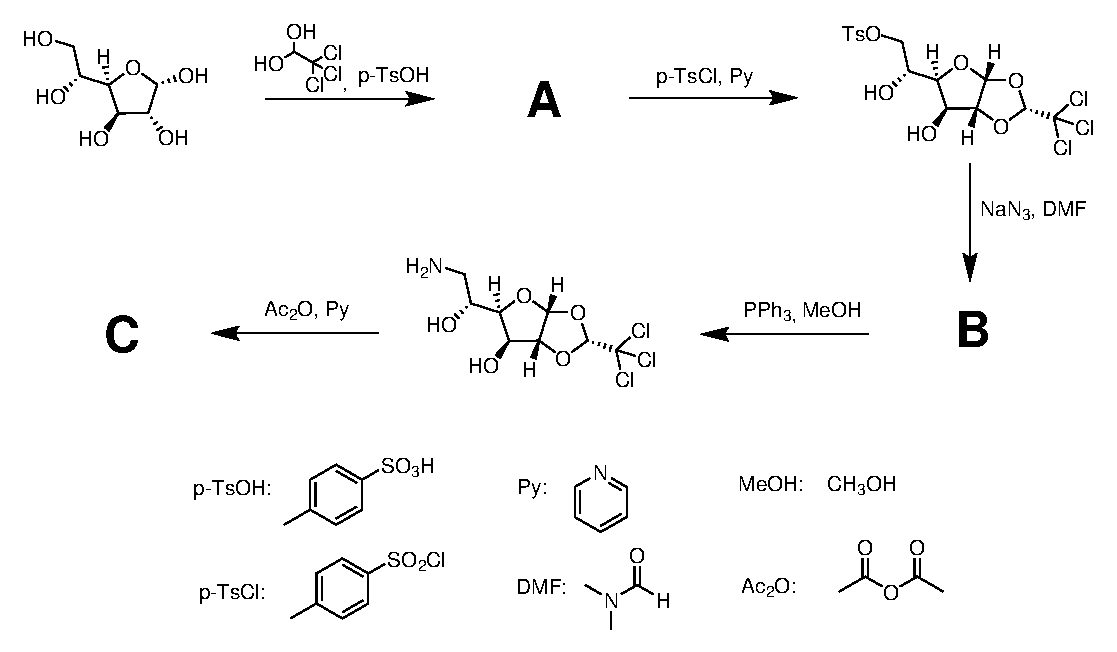
\includegraphics[width=\textwidth]{2024/Abbildungen/Hydrat/Synthesesquenz.eps}
\end{figure}


\enumaufgabe{\operator{Gib} die Strukturformeln der Verbindungen A, B und C unter Berücksichtigung der Stereochemie \operator{an}.}

\begin{tabularx}{\textwidth}{|X|X|}\hline
     \textbf{A} \solutiontext{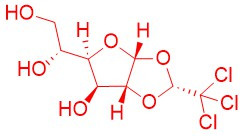
\includegraphics[width=0.3\textwidth]{2024/Abbildungen/Hydrat/A.jpg}
     }{\vspace{4cm}} & \textbf{B}      \solutiontext{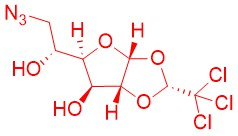
\includegraphics[width=0.3\textwidth]{2024/Abbildungen/Hydrat/B.jpg}}{\vspace{4cm}}\\\hline
     \textbf{C} \solutiontext{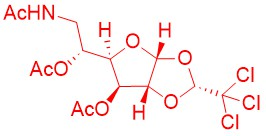
\includegraphics[width=0.3\textwidth]{2024/Abbildungen/Hydrat/C.jpg}
     }{\vspace{4cm}} &\\\hline
\end{tabularx}
\solutiontext{2 P. für richtige Strukturformel, 0,5 P. für korrekte Stereochemie\\
insg. 7,5 P.}{}\\
\solutiontext{$\sum$ 40,5 P.}{}
\end{document}